\documentclass[handout]{beamer}
\usetheme{default}
\usepackage{tikz}
\usetikzlibrary{positioning}
\setbeamertemplate{footline}[page number]
\setbeamertemplate{navigation symbols}{}
\usepackage{hyperref}
\usepackage{listings}
\lstset{language=C}
\newcommand{\todo}[1]{{\tt ... #1 ... }}
\newcommand{\Reach}{\mathrm{Reach}}
\newcommand{\Path}{\mathrm{path}}

%Stolen from Stackexchange
%http://tex.stackexchange.com/questions/20609/strikeout-in-math-mode 
\newcommand\hcancel[2][red]{\setbox0=\hbox{$#2$}%
\rlap{\raisebox{.45\ht0}{\textcolor{#1}{\rule{\wd0}{1pt}}}}#2} 

\title{Software Testing\\ Lecture 3\\ Coverage}
\author{Justin Pearson}
\date{2017}
\setbeamertemplate{footline}[page number]
\setbeamertemplate{navigation symbols}{}

\begin{document}
\lstset{language=C}

\begin{frame}
  \maketitle
\end{frame}

\begin{frame}{Approaches to testing}
  \begin{itemize}
  \item Black Box Testing: Test without looking at the code/hardware
  \item White Box Testing (clear box testing):  Test the internal
    structure of the software
  \end{itemize}
  There is also grey box testing where you look find test cases that cover the
  specification and cover some aspect of the code.  It is a grey area.  
\end{frame}
\begin{frame}{It is all about coverage}
  \begin{itemize}
  \item Black box testing: test by covering the specification
  \item White box testing: test by covering the source code
    \begin{itemize}
    \item Execution paths
    \item Statements
    \item Decision coverage
    \item $\ldots$
    \end{itemize}
  \end{itemize}
  Short version:
  \begin{itemize}
  \item  Complete coverage hard to define or impossible;
  \item  So we have to find some approximation.
  \end{itemize}
\end{frame}

\begin{frame}[fragile]{Turing's halting problem}
Does this program halt?
\begin{lstlisting}
  main() {
   int i=0;
   int z=0;
   for(i=0; i<10; i++) {
     z = z + 1;
   }
  }
\end{lstlisting}
\end{frame}
\begin{frame}[fragile]{Turing's halting problem}
Does this program halt?
\begin{lstlisting}
  main() {
   int i=0;
   int z=0;
   while(1 != 0) {
     z = z + 1;
   }
  }
\end{lstlisting}
\end{frame}

\begin{frame}{Turing's halting problem}
  \begin{itemize}
  \item Can I write  a program that takes {\em any} program and
    decides if it halts?
  \end{itemize}
  Seems that is might be possible, but it is mathematically impossible.

 
\end{frame}
\begin{frame}{Turing's halting problem}
Proof
  \begin{itemize}
  \item  Enumerate all programs. There are infinitely many, but still
    a countable number\footnote{You can put them in an infinitely long list.}.
  \item Give each program a number. 
  \item The function
    \[
      h(i,x) = \begin{cases}
               1 & \text{if program i halts on input x} \\
               0 & \text{otherwise}
               \end{cases}
    \]
is not computable. That is there no always halting program that implements
$h$. 
  \end{itemize}
\end{frame}
\begin{frame}
  \begin{itemize}
  \item   Given
    \[
      h(i,x) = \begin{cases}
               1 & \text{if program i halts on input x} \\
               0 & \text{otherwise}
               \end{cases}
    \]
  \item Define
    \[
    g(i) = \begin{cases}
             0 & \text{if $h(i,i) = 0$} \\
             \text{loop forever} & \text{otherwise}
           \end{cases}
    \]
\item $g$ is a program it has a number, lets call it $\mathcal{G}$.
\item What of $h(\mathcal{G},\mathcal{G})$? Two possibilities:
  \begin{itemize}
  \item  $h(\mathcal{G},\mathcal{G}) = 1$ \pause then $g$ halts on input $\mathcal{G}$, so $g(\mathcal{G})=0$ which
    implies $h(\mathcal{G},\mathcal{G}) =  0$, hence a contradiction. \pause
  \item $h(\mathcal{G},\mathcal{G}) = 0$ \pause then $g$ loops for ever on input $g$. Which implies
    $h(\mathcal{G},\mathcal{G})$ is not equal to 0, hence contradiction.
  \end{itemize}
  \end{itemize}
Proof strategy is often referred to as a diagonal argument. 
\end{frame}
\begin{frame}{Common Caveats}
  \begin{itemize}
  \item Halting function should work on \textcolor{red}{\em all} programs.
  \item Finite memory, finite number of registers a computer is just a
    finite state machine.
  \item So it is possible to write a function that decides if all
    programs up to a given size terminate, but not very efficiently.
  \item Also knowing that the program halts for all memory sizes up to
    certain value does not necessarily tell you anything about bigger
    sizes. 
\item How big is big enough? 
  \end{itemize}
\end{frame}
\begin{frame}{Rice's Theorem}
  \begin{itemize}
  \item All interesting properties are non-computable. 
  \item Ask yourself: Is what I'm trying to do equivalent to the
    halting problem?
    \item Are all execution paths covered?
      \begin{itemize}
      \item  If you could solve that problem, then you would solve the
        halting problem.
      \end{itemize}
    \item This is the origin of 
  \begin{quote}
    ``Program testing can be used to show the presence of bugs, but
    never to show their absence!'' Edsger Dijkstra.
  \end{quote}
  \end{itemize}
\end{frame}
\begin{frame}{Pragmatics}
  \begin{itemize}
  \item Admit we can not decide properties on all programs.
  \item Do our best on most programs.
  \item Or be content with approximations such as: 
    \begin{itemize}
    \item Definitely yes
    \item Definitely no
    \item I have no idea.
    \end{itemize}
  \end{itemize}
\end{frame}
\begin{frame}{White Box testing}
Coverage criteria include:
  \begin{itemize}
  \item Function coverage --- Has each function (or subroutine) in the
    program been called?
  \item Statement coverage --- Has each statement in the program been
    executed?  
  \item Branch coverage --- Has each branch of each control structure
    (such as in {\tt if} and {\tt case} statements) been executed?
  \item Loop coverage --- Have we done a representative number of iterations
    of all the loops. 
  \end{itemize}
\end{frame}

\begin{frame}[fragile]{Statement and Branch coverage}

\begin{itemize}
\item Statement coverage $\subseteq$ Branch coverage
\begin{lstlisting}
       silly(int x) {
         int y=0;
         if (x==1) {
           y=100;
         }
         twonk(y);
       }
\end{lstlisting}

  \item  The test case {\tt silly(1)} covers all statements in the program, but
  it does not cover all branches. We never test the case when {\tt x}$\neq1$.
\end{itemize}
\end{frame}

\begin{frame}[fragile]{Statement and Branch coverage}
\begin{itemize}
 \item Even branch coverage is a blunt instrument.
\begin{lstlisting}
   int silly(int x) { 
      int y=0;
      while (x >= 0) {
         y = y + x;
         x--
        }
      return(y);
   }
\end{lstlisting}
  \item The test case {\tt silly(1)} runs the loop once. A while loop is a
    branch with a goto statement. 
  \item But what about running the loop zero times, lots of times?
   \item Halting problem again, for all most all loop you can't
     decide how many times to run the loop.
\end{itemize}
    
\end{frame}
%%%%You are here, be pragmatic, how much to talk about graphs.

 \begin{frame}{Control Flow Graphs}

Control flow graphs models the control structures of the program. We
can use them to reason about executions and test cases.
\begin{itemize}
\item Nodes: Statements of sequence of statements
\item Edges: Transfer of control
\item Basic Block: Sequence of statements with no transfer of control.
\end{itemize}
\end{frame}


\begin{frame}[fragile]%{If statement}
\frametitle{If statements}
\begin{columns}
\begin{column}{0.5\textwidth}
\begin{lstlisting}
         if (x<y) 
         { 
           y=0; 
         } else
         {
           x=y;
         }
\end{lstlisting}
\end{column}
\begin{column}{0.5\textwidth}
 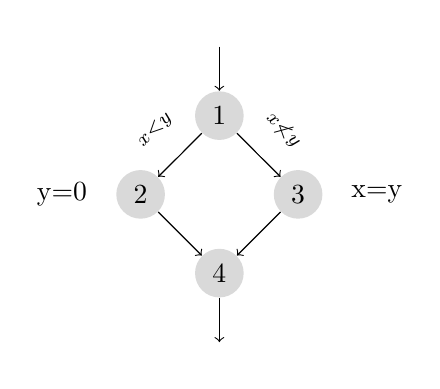
\begin{tikzpicture}
 \node (entry) at (1,3) {};
 \node (exit) at (1,-1) {};
 \node (text1) at (-1,1) {y=0};
 \node (text2) at (3,1) {x=y};
 \tikzstyle{every node} = [circle,fill=gray!30]
 \node (a) at (1,2) {1};
 \node (b) at (0,1) {2};
 \node (c) at (2,1) {3};
 \node (d) at (1,0) {4};
 \draw [->] (entry) to (a);
 \draw [->] (a)  -- node[color=black,fill=white,pos=0.5,sloped,above] {$
   \scriptstyle x<y$} (b);
 \draw [->] (a)  -- node[color=black,fill=white,pos=0.5,sloped,above]
 {$\scriptstyle x \not <
   y$} (c);
 \draw [->] (c) to (d);
 \draw [->] (b) to (d);
 \draw [->] (d) to (exit);
\end{tikzpicture}
\end{column}
\end{columns}
\end{frame}

\begin{frame}[fragile]%{If statement}
\frametitle{If statements}
\begin{columns}
\begin{column}{0.5\textwidth}
\begin{lstlisting}
         if (x<y) 
         { 
           y=0; 
         };

\end{lstlisting}
\end{column}
\begin{column}{0.5\textwidth}
 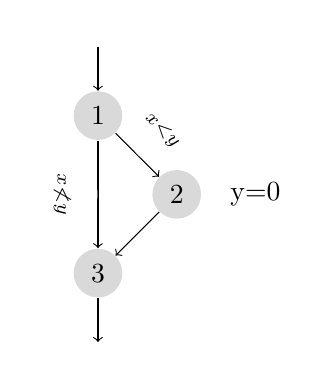
\begin{tikzpicture}
 \node (entry) at (1,3) {};
 \node (exit) at (1,-1) {};
 \node (text2) at (3,1) {y=0};
 \tikzstyle{every node} = [circle,fill=gray!30]
 \node (a) at (1,2) {1};
 \node (c) at (2,1) {2};
 \node (d) at (1,0) {3};
 \draw [->] (entry) to (a);
 \draw [->] (a)  -- node[color=black,fill=white,pos=0.5,sloped,above] {$
   \scriptstyle x<y$} (c);
 \draw [->] (a)  -- node[color=black,fill=white,pos=0.5,sloped,below]
 {$\scriptstyle x \not <
   y$} (d);
 \draw [->] (c) to (d);
 \draw [->] (d) to (exit);
\end{tikzpicture}
\end{column}
\end{columns}
\end{frame}

\begin{frame}[fragile]%{If statement}
\frametitle{If return statements}
\begin{columns}
\begin{column}{0.5\textwidth}
\begin{lstlisting}
         if (x<y) 
         { 
           return;
         }
         print(x);
         return;
\end{lstlisting}
\end{column}
\begin{column}{0.5\textwidth}
 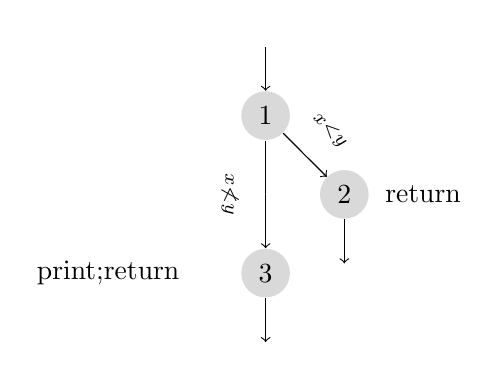
\begin{tikzpicture}
 \node (entry) at (1,3) {};
 \node (exit) at (1,-1) {};
 \node (exit2) at (2,0) {};
 \node (text2) at (3,1) {return};
 \node (text3) at (-1,0) {print;return};
 \tikzstyle{every node} = [circle,fill=gray!30]
 \node (a) at (1,2) {1};
 \node (c) at (2,1) {2};
 \node (d) at (1,0) {3};
 \draw [->] (entry) to (a);
 \draw [->] (a)  -- node[color=black,fill=white,pos=0.5,sloped,above] {$
   \scriptstyle x<y$} (c);
 \draw [->] (a)  -- node[color=black,fill=white,pos=0.5,sloped,below]
 {$\scriptstyle x \not <
   y$} (d);
 \draw [->] (d) to (exit);
 \draw [->] (c) to (exit2);
\end{tikzpicture}
\end{column}
\end{columns}
Note that we do not collapse the two return statements. 
\end{frame}

\begin{frame}[fragile]{Loops}
\begin{columns}
\begin{column}{0.5\textwidth}
\begin{lstlisting}
  for(i=0; i<x; i++) {
    loop_body();
  }
\end{lstlisting}
\end{column}
\begin{column}{0.5\textwidth}
 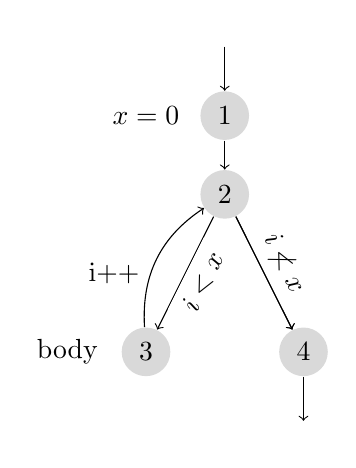
\begin{tikzpicture}
 \node (entry) at (1,3) {};
 
% \tikzstyle{every node} = [circle,fill=gray!30]
 \node[below of=entry,circle,fill=gray!30] (initialise) {$1$};
 \node[left  of=initialise] () {$x=0$};
 \node[below of=initialise,circle,fill=gray!30] (start) {$2$};
 \node[below of=start] (placementnode) {};
 \node[left of=placementnode, below of=placementnode,circle,fill=gray!30] (body)
 {$3$}; 
 \node[left of=body] () {body};
 \node[left of=placementnode,node distance=4em] (anchorpoint) {i++};
 \node[right of=placementnode, below of=placementnode,circle,fill=gray!30] (exit)
{$4$};
 \node[below of=exit] (exitnode) {};
 
 \draw [->] (exit) to (exitnode);
 \draw [->] (entry) to (initialise);
 \draw [->] (initialise) to (start);
 \draw [->] (start) --
 node[color=black,fill=white,pos=0.5,below,sloped] {$\scriptsize i<x$}
 (body);
 \draw [->] (start) --
 node[color=black,fill=white,pos=0.5,above,sloped] {$\scriptsize i\not<x$} (exit);
 \draw [->] (start) to (exit);
  \draw [->] (body) to[bend left] (start);
\end{tikzpicture}
\end{column}
\end{columns}
\end{frame}

\begin{frame}
  \begin{itemize}
  \item Other program constructs are easy to do.
  \item Each node only to be labelled with one basic block.
  \item Beware of hidden control structures. (C's case statement).
  \end{itemize}
\end{frame}
 \begin{frame}{Paths}
Other definitions possible.
   \begin{itemize}
   \item A path is a sequence of nodes.
   \item The length of a path is the number of edges. A path with only
     one node, hence no edge has length $0$.
   \item Subpath is sub-sequence of a path.
   \item $\Reach(n)$  the set of nodes that can be reach via  a
     directed path from the node $n$.
   \end{itemize}
 \end{frame}

 \begin{frame}{Paths}
       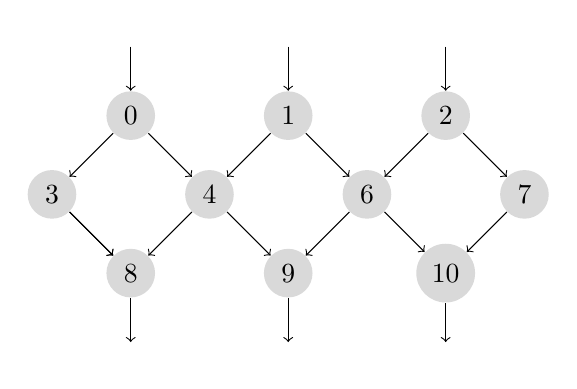
\begin{tikzpicture}
         \node (entry1) at (1,3) {} ;
     \node (entry2) at (3,3) {} ;
     \node (entry3) at (5,3) {};
     \node (exit1) at (1,-1) {} ;
     \node (exit2) at (3,-1) {} ;
     \node (exit3) at (5,-1) {} ;
     \tikzstyle{every node} = [circle,fill=gray!30]
     \node (a1) at (1,2) {0};
     \node (a2) at (3,2) {1};
     \node (a3) at (5,2) {2};
     \node (b1) at (0,1) {3};
     \node (b2) at (2,1) {4};
     \node (c2) at (4,1) {6};
     \node (c3) at (6,1) {7};
     \node (d1) at (1,0) {8};
     \node (d2) at (3,0) {9};
     \node (d3) at (5,0) {10};
     \draw [->] (entry1) to (a1);
     \draw [->] (entry2) to (a2);
     \draw [->] (entry3) to (a3);
     \draw [->] (a1) to (b1);
     \draw [->] (a1) to (b2);
     \draw [->] (b2) to (d1);
     \draw [->] (b1) to (d1);
     \draw [->] (b1) to (d1);
     \draw [->] (d1) to (exit1);
     \draw [->] (a2) to (b2);
     \draw [->] (a2) to (c2);
     \draw [->] (c2) to (d2);
     \draw [->] (b2) to (d2);
     \draw [->] (d2) to (exit2);
     \draw [->] (a3) to (c2);
     \draw [->] (a3) to (c3);
     \draw [->] (c3) to (d3);
     \draw [->] (c2) to (d3);
     \draw [->] (d3) to (exit3);
   \end{tikzpicture}
   \begin{itemize}
   \item Paths include: $[0,3,8],[0,4,8],[0,4,9],[1,4,8],\ldots ,
     [4,8], \ldots$.
   \end{itemize}
 \end{frame}
 \begin{frame}{$\Reach(n)$}
       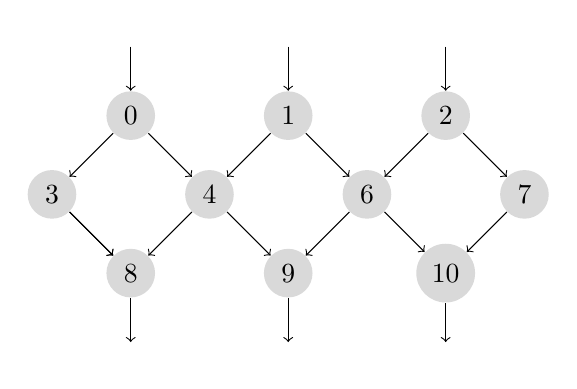
\begin{tikzpicture}
         \node (entry1) at (1,3) {} ;
     \node (entry2) at (3,3) {} ;
     \node (entry3) at (5,3) {};
     \node (exit1) at (1,-1) {} ;
     \node (exit2) at (3,-1) {} ;
     \node (exit3) at (5,-1) {} ;
     \tikzstyle{every node} = [circle,fill=gray!30]
     \node (a1) at (1,2) {0};
     \node (a2) at (3,2) {1};
     \node (a3) at (5,2) {2};
     \node (b1) at (0,1) {3};
     \node (b2) at (2,1) {4};
     \node (c2) at (4,1) {6};
     \node (c3) at (6,1) {7};
     \node (d1) at (1,0) {8};
     \node (d2) at (3,0) {9};
     \node (d3) at (5,0) {10};
     \draw [->] (entry1) to (a1);
     \draw [->] (entry2) to (a2);
     \draw [->] (entry3) to (a3);
     \draw [->] (a1) to (b1);
     \draw [->] (a1) to (b2);
     \draw [->] (b2) to (d1);
     \draw [->] (b1) to (d1);
     \draw [->] (b1) to (d1);
     \draw [->] (d1) to (exit1);
     \draw [->] (a2) to (b2);
     \draw [->] (a2) to (c2);
     \draw [->] (c2) to (d2);
     \draw [->] (b2) to (d2);
     \draw [->] (d2) to (exit2);
     \draw [->] (a3) to (c2);
     \draw [->] (a3) to (c3);
     \draw [->] (c3) to (d3);
     \draw [->] (c2) to (d3);
     \draw [->] (d3) to (exit3);
   \end{tikzpicture}   
   \begin{itemize}
   \item $\Reach(3) = \{8\}$, $\Reach(1) = \{4,9,8,6,10\}$.
   \end{itemize}
 \end{frame}
%%%%%%%%
\begin{frame}[fragile]{Reach}
  \begin{itemize}
  \item Two notions in program analysis:
    \begin{itemize}
    \item Syntactic reach. 
    \item Semantic Reach.
    \end{itemize}
   \end{itemize}
\begin{lstlisting}
      main() {
        for(i=0; true; i++) {
          if (f(i) == 0) { break(0);}
        }
        X();
      }
\end{lstlisting}
%%%
{\tt X()}  is syntactically reachable, but
semantically you have to infer something about {\tt f()}.
\end{frame}
%%%%%%%
\begin{frame}{Test Path}
   \begin{itemize}
   \item  A test path starts at an initial node and ends in a final
     node.
   \item Test paths represent execution of test cases.
     \begin{itemize}
     \item  Some paths can be executed by many test cases.
     \item Some paths can not be executed by any test cases (halting
       problem again).
     \end{itemize}
   \end{itemize}
\end{frame}
%%%%%%%
 \begin{frame}{Test and Test Paths}
\begin{center}
   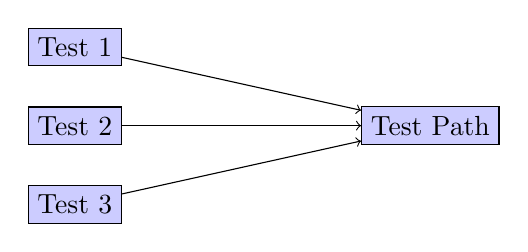
\begin{tikzpicture}
     \node[rectangle,draw,fill=blue!20] (test1) {Test 1};
     \node[rectangle,below of=test1,draw,fill=blue!20] (test2) {Test 2};
     \node[rectangle,below of=test2,draw,fill=blue!20] (test3) {Test
       3};
     \node[right of=test2,node distance=10em]  (placementnode) {};
     \node[rectangle,right of=placementnode,draw,fill=blue!20] (path)
     {Test Path};
     \draw [->] (test1) to (path);
     \draw [->] (test2) to (path);
     \draw [->] (test3) to (path);
   \end{tikzpicture}
\end{center}
Many to one. Deterministic software, each test path has identical
execution.
\begin{center}
   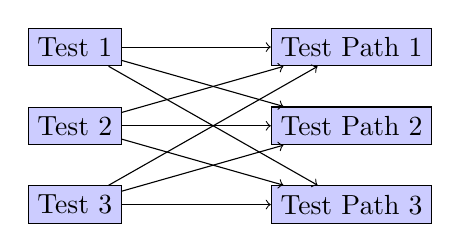
\begin{tikzpicture}
     \node[rectangle,draw,fill=blue!20] (test1) {Test 1};
     \node[rectangle,below of=test1,draw,fill=blue!20] (test2) {Test 2};
     \node[rectangle,below of=test2,draw,fill=blue!20] (test3) {Test
       3};
     \node[rectangle,right of=test1,draw,fill=blue!20,node
     distance=10em] (path1) {Test Path 1};
     \node[rectangle,right of=test2,draw,fill=blue!20,node
          distance=10em] (path2) {Test Path 2};
     \node[rectangle,right of=test3,draw,fill=blue!20,node
     distance=10em] (path3) {Test Path 3};
     \draw[->] (test1) to (path1);
     \draw[->] (test1) to (path2);
     \draw[->] (test1) to (path3);
     \draw[->] (test2) to (path1);
     \draw[->] (test2) to (path2);
     \draw[->] (test2) to (path3);
     \draw[->] (test3) to (path1);
     \draw[->] (test3) to (path2);
     \draw[->] (test3) to (path3);
   \end{tikzpicture}
\end{center}
Many to many, non-deterministic software (you'll meet it all the time)
a test can execute many test paths.
 \end{frame}
 \begin{frame}{Testing and Covering Graphs}
   \begin{itemize}
   \item {\em Test Requirements (TR)} : Describe properties of test paths
     \item {\em Test Criterion} : Rules that define test requirements
     \item {\em Satisfaction} : Given a set TR of test requirements
       for a criterion $C$, a set of tests $T$ satisfies C on a graph if
       and only if for every test requirement in TR, there is a test
       path in $\Path(T)$ that meets the test requirement.
   \end{itemize}
General idea in testing. Define your test requirements separately from
the tests cases. Reformulate your requirements  into test
criteria and then try to find test paths that satisfy your test
criteria.
 \end{frame}

\begin{frame}{Node Coverage --- Statement Coverage} 
  \begin{itemize}
  \item Node Coverage (NC) : Test set $T$ satisfies node coverage on
    graph $G$ iff for every syntactically reachable node $n$ in $N$, there
    is some path $p$ in path($T$) such that $p$ visits $n$.
  \end{itemize}
\end{frame}
\begin{frame}{Edge Coverage --- Branch Coverage}
  \begin{itemize}
  \item Edge Coverage (EC) : TR contains each reachable path of length
    up to 1, inclusive, in $G$.
  \end{itemize}
Is there any difference between node and edge coverage?
\end{frame}
\begin{frame}{Difference between node and edge coverage}
 \begin{columns}
   \begin{column}{0.5\textwidth}
     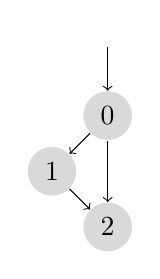
\begin{tikzpicture}
       \node (start) {};
       \node [below of=start,circle,fill=gray!30] (i) {$0$};
       \node [below left of=i,circle,fill=gray!30] (a) {$1$};
       \node [below right of=a,circle,fill=gray!30] (b) {$2$};
       \draw [->] (start) to (i);
       \draw [->] (i) to (a);
       \draw [->] (i) to (b);
       \draw [->] (a) to (b);
     \end{tikzpicture}
   \end{column}
   \begin{column}{0.5\textwidth}
     \begin{itemize}
     \item Node coverage
       \begin{itemize}
       \item Test requirement (TR) = $\{0,1,2\}$.
       \item Test path = $[0,1,2]$.
       \end{itemize}
     \item Edge Coverage
       \begin{itemize}
       \item Test requirement (TR) = $\{(0,1),(0,2),(1,2)\}$.
       \item Test paths = $[0,1,2],[0,2]$.
       \end{itemize}
     \end{itemize}
   \end{column}
 \end{columns}
\end{frame}
\begin{frame}{Complete Path Coverage}
  \begin{itemize}
  \item Require that all paths are covered.
  \end{itemize}
  Often there are too many paths. So various approximations.
  \begin{itemize}
  \item Require that all paths up to length $k$ are covered.
    \begin{itemize}
    \item $k=0$, node coverage.
    \item $k=1$, edge coverage.
    \item $k=2$, edge pair coverage.
    \end{itemize}
  \end{itemize}
\end{frame}

 \begin{frame}{Structural Coverage Example}
  \begin{columns}
    \begin{column}{0.2\textwidth}
      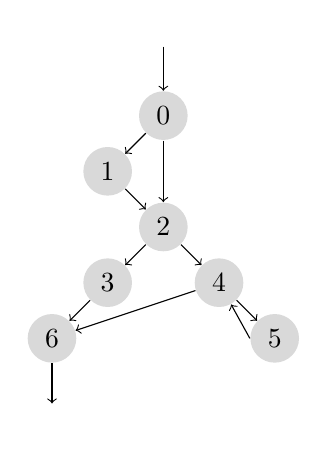
\begin{tikzpicture}
        \node (entry) {};
        \tikzstyle{every node} = [circle,fill=gray!30]
        \node[below of=entry] (a) {0};
        \node[below left of=a] (b) {1};
        \node[below right of=b] (c) {2};
        \node[below left of=c] (d) {3};
        \node[below right of=c] (e) {4};
        \node[below left of=d] (f) {6};
        \node[below right of=e] (g) {5};
        \node[draw=none,fill=none,below of=f] (exit) {};
        \draw[->] (entry) to (a);
        \draw[->] (a) to (b);
        \draw[->] (a) to (c);
        \draw[->] (b) to (c);
        \draw[->] (c) to (d);
        \draw[->] (c) to (e);
        \draw[->] (d) to (f);
        \draw[->] (e) to (f);
        \draw[->] (e) to (g);
        \draw[->] (g.west) to (e);
        \draw[->] (f) to (exit);
      \end{tikzpicture}
    \end{column}
    \begin{column}{0.8\textwidth}
      \begin{itemize}
      \item Node Coverage: $TR=\{0,1,2,3,4,5,6\}$, test paths =
        $\{[0,1,2,3,6],[0,1,2,4,5,4,6]\}$.
      \item Edge Coverage:
        $TR=\{(0,1),(0,2),(1,2),(2,3),(2,4),(3,6),(4,5),(4,6),(5,4)\}$,
        Test paths $[0,1,2,3,6]$, $[0,2,4,5,4,6]$.
%      \item Edge-Pair Coverage: $TR=\{[0,1,2],[0,2,3],[0,2,4],[1,2,3],[1,2,4],[2,3,6],[2,4,5]$,$[2,4,6],[4,5,4],[5,4,5],[5,4,6]\}$.
      \item Complete Path Coverage. Test paths
        $[0,1,2,3,6]$,$[0,1,2,4,6]$,$[0,1,2,4,5,4,6]$, $[0,1,2,4,5,4,5,4,6]$, etc.
      \end{itemize}
    \end{column}
  \end{columns}
\end{frame}

\begin{frame}{Structural Coverage Example}
  \begin{columns}
    \begin{column}{0.2\textwidth}
      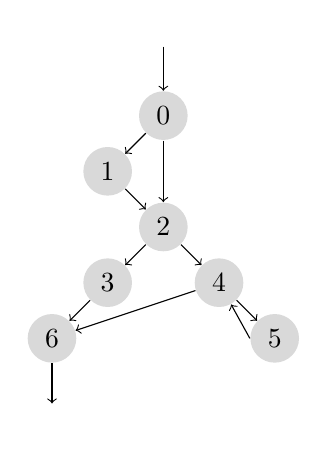
\begin{tikzpicture}
        \node (entry) {};
        \tikzstyle{every node} = [circle,fill=gray!30]
        \node[below of=entry] (a) {0};
        \node[below left of=a] (b) {1};
        \node[below right of=b] (c) {2};
        \node[below left of=c] (d) {3};
        \node[below right of=c] (e) {4};
        \node[below left of=d] (f) {6};
        \node[below right of=e] (g) {5};
        \node[draw=none,fill=none,below of=f] (exit) {};
        \draw[->] (entry) to (a);
        \draw[->] (a) to (b);
        \draw[->] (a) to (c);
        \draw[->] (b) to (c);
        \draw[->] (c) to (d);
        \draw[->] (c) to (e);
        \draw[->] (d) to (f);
        \draw[->] (e) to (f);
        \draw[->] (e) to (g);
        \draw[->] (g.west) to (e);
        \draw[->] (f) to (exit);
      \end{tikzpicture}
    \end{column}
    \begin{column}{0.8\textwidth}
      \begin{itemize}
      \item Edge-Pair Coverage: $TR=\{[0,1,2],[0,2,3]$,
        $[0,2,4],[1,2,3],[1,2,4]$,$[2,3,6]$, $[2,4,5]$,$[2,4,6]$,
        $[4,5,4],[5,4,5],[5,4,6]\}$
      \item Test Paths
        \begin{itemize}
        \item $[0,1,2,3,6]$,$[0,1,2,4,6]$, $[0,2,3,6]$
        \item $[0,2,4,5,4,5,4,6]$.
        \end{itemize}
      \end{itemize}
    \end{column}
  \end{columns}
\end{frame}




\begin{frame}
  \frametitle{Summary}
  \begin{itemize}
  \item Turing's halting theorem tells us that in a strong sense that testing
    for correctness is impossible.
  \item Formalising programs as control flow graphs gives us a way to talk
    about testing.
  \item Node coverage corresponds to statement coverage, edge coverage
    corresponds to something like branch coverage. Covering all execution
    paths is impossible with loops, so there are various approximations.
  \end{itemize}
  Don't forget the distinction between syntactic and semantic reachability. 
\end{frame}

\end{document}

%%% Local Variables:
%%% mode: latex
%%% TeX-master: t
%%% End:
